
\section{Syntax}

As we did whit multi $\pi$ calculus, we suppose that we have a countable set of names $\mathbb{N}$, ranged over by lower case letters $a,b, \cdots, z$. This names are used for communication channels and values. Furthermore we have a set of identifiers, ranged over by $A$. We represent the agents or processes by upper case letters $P,Q, \cdots $. A multi $\pi$ process, in addiction to the same actions of a $\pi$ process, can perform also a strong prefix:
\begin{center}
  $\pi$ ::= $\overline{x}y$ | $x(z)$ | $\underline{x(y)}$ | $\underline{\overline{x}y}$ |$\tau$ 
\end{center}
The process are defined, just as original $\pi$ calculus, by the following grammar:
\begin{center}
  \begin{tabular}{l}
    $P,Q$ ::= $0$ | $\pi.P$ | $P|Q$ | $P+Q$ | $(\nu x) P$ | $A(y_{1}, \cdots, y_{n})$
  \end{tabular}
\end{center}
and they have the same intuitive meaning as for the $\pi$ calculus. The strong prefix input allows a process to make an atomic sequence of actions, so that more than one process can synchronize on this sequence. 

We have to extend the following definition to deal with the strong prefix:
\begin{center}
  \begin{tabular}{ll}
	$B(\underline{x(y)}.Q, I)\; =\; \{y,\overline{y}\}\cup B(Q, I)$
      &
	$F(\underline{x(y)}.Q, I)\; =\; \{x,\overline{x}\}\cup (F(Q, I)-\{y,\overline{y}\})$
    \\
	$B(\underline{\overline{x}y}.Q, I)\; =\; B(Q,I)$
      &
	$F(\underline{\overline{x}y}.Q, I)\; =\; \{x,\overline{x},y,\overline{y}\}\cup F(Q, I)$
    \\
  \end{tabular}
\end{center}

\section{Operational semantic}
\subsection{Early operational semantic with structural congruence}

\subsection{Late operational semantic with structural congruence}

The semantic of a multi $\pi$ process is labeled transition system such that
\begin{itemize}
  \item 
    the nodes are multi $\pi$ calculus process. The set of node is $\mathbb{P}_{m}$
  \item
    The set of actions is $\mathbb{A}_{m}$ and can contain
    \begin{itemize}
      \item 
	bound output $\overline{x}(y)$
      \item
	unbound output $\overline{x}y$ 
      \item
	bound input $x(z)$
    \end{itemize}
    We use $\alpha, \alpha_{1}, \alpha_{2},\cdots $ to range over the set of actions, we use $\sigma, \sigma_{1}, \sigma_{2}, \cdots $ to range over the set $\mathbb{A}_{m}^{+} \cup \{\tau\}$. 
  \item
    the transition relations is $\rightarrow\subseteq \mathbb{P}_{m}\times (\mathbb{A}_{m}^{+} \cup \{\tau\})\times \mathbb{P}_{m}$
\end{itemize}

In this case, a label can be a sequence of prefixes, whether in the original $\pi$ calculus a label can be only a prefix. We use the symbol $\cdot$ to denote the concatenation operator.

% \begin{definition}\index{transition relation! multipi! late! with structural congruence}
%   The \emph{late transition relation with structural congruence} is the smallest relation induced by the rules in table \ref{multiIOlatewith1}
%   \begin{table}
%     \begin{tabular}{ll}
% 	  \hline\\
%  	  \bf{Pref}
%  	  \begin{tabular}{c}
%  	      $\alpha\; not\; a\; strong\; prefix$
%  	    \\\hline
%  	      $\alpha.P \;\xrightarrow{\alpha} P$
%  	  \end{tabular}
% 	&
% 	  \bf{Par}
% 	  \begin{tabular}{c}
% 	      $P \;\xrightarrow{\sigma} P^{'}\;\; bn(\sigma)\cap fn(Q)=\emptyset$
% 	    \\\hline
% 	      $P|Q \;\xrightarrow{\sigma} P^{'}|Q$
% 	  \end{tabular}
%       \\\\
% 	  \bf{SOut}
% 	  \begin{tabular}{c}
% 	      $P \;\xrightarrow{\sigma} P^{'}\;\; \sigma\neq \tau$
% 	    \\\hline
% 	      $\underline{\overline{x}y}.P \;\xrightarrow{\overline{x}y \cdot \sigma} P^{'}$
% 	  \end{tabular}
% 	&
% 	  $\inferrule* [left=\bf{LComSeq1}]{
% 	      P \;\xrightarrow{x(y)}\; P^{'}
% 	    \\
% 	      Q\;\xrightarrow{\overline{x}z\cdot \sigma} Q^{'}
% 	    \\
% 	      z\notin fn(P)
% 	  }{
% 	    P|Q \;\xrightarrow{\sigma} P^{'}\{z/y\}|Q^{'}
% 	  }$
%       \\\\
% 	  \bf{Sum}
% 	  \begin{tabular}{c}
% 	      $P \;\xrightarrow{\sigma} P^{'}$
% 	    \\\hline
% 	      $P+Q \;\xrightarrow{\sigma} P^{'}$
% 	  \end{tabular}
% 	&
% 	$\inferrule* [left=\bf{Str}]{
% 	    P\equiv P^{'}
% 	  \\
% 	    P^{'}\; \;\xrightarrow{\alpha}\; Q^{'}
% 	  \\
% 	    Q\equiv Q^{'}
% 	}{
% 	    P\; \;\xrightarrow{\alpha}\; Q
% 	}$
%       \\\\
% 	  \bf{Res}
% 	  \begin{tabular}{c}
% 	      $P \;\xrightarrow{\sigma} P^{'}\;\; z\notin n(\alpha)$
% 	    \\\hline
% 	      $(\nu z) P \;\xrightarrow{\sigma} (\nu z) P^{'}$
% 	  \end{tabular}
% 	&
% 	  $\inferrule* [left=\bf{LComSng}]{
% 	      P \;\xrightarrow{x(y)} P^{'}
% 	    \\
% 	      Q\;\xrightarrow{\overline{x}z} Q^{'}
% 	    \\
% 	      z\notin fn(P)
% 	  }{
% 	    P|Q \;\xrightarrow{\tau} P^{'}\{z/y\}|Q^{'}
% 	  }$
%       \\\\
% 	  $\inferrule* [left=\bf{SInp}]{
% 	      P \;\xrightarrow{\sigma}\; P^{'}
% 	    \\
% 	      \sigma\neq \tau
% 	  }{
% 	    \underline{x(y)}.P \;\xrightarrow{x(y) \cdot \sigma} P^{'}
% 	  }$
% 	&
% 	  $\inferrule* [left=\bf{LComSeq2}]{
% 	      P \;\xrightarrow{\overline{x}z}\; P^{'}
% 	    \\
% 	      Q\;\xrightarrow{x(y)\cdot \sigma}\; Q^{'}
% 	    \\
% 	      z\notin fn(P)
% 	  }{
% 	    P|Q \;\xrightarrow{\sigma\{z/y\}}\; P^{'}|Q^{'}\{z/y\}
% 	  }$
%       \\\hline
%     \end{tabular}
%     \caption{Multi $\pi$ late semantic with structural congruence}
%     \label{multiIOlatewith1}
%   \end{table}
% \end{definition}


% \subsection{Another attemp to late operational semantic with structural congruence}

\begin{definition}\index{transition relation! multipi! late! with structural congruence}
  The \emph{late transition relation with structural congruence} is the smallest relation induced by the rules in table \ref{multiIOlatewith2}:
  \begin{table}
    \begin{tabular}{ll}
	  \hline\\
 	  \bf{Pref}
 	  \begin{tabular}{c}
 	      $\alpha\; not\; a\; strong\; prefix$
 	    \\\hline
 	      $\alpha.P \;\xrightarrow{\alpha} P$
 	  \end{tabular}
	&
	  \bf{Par}
	  \begin{tabular}{c}
	      $P \;\xrightarrow{\sigma} P^{'}\;\; bn(\sigma)\cap fn(Q)=\emptyset$
	    \\\hline
	      $P|Q \;\xrightarrow{\sigma} P^{'}|Q$
	  \end{tabular}
      \\\\
	  \bf{SOut}
	  \begin{tabular}{c}
	      $P \;\xrightarrow{\sigma} P^{'}\;\; \sigma\neq \tau$
	    \\\hline
	      $\underline{\overline{x}y}.P \;\xrightarrow{\overline{x}y \cdot \sigma} P^{'}$
	  \end{tabular}
	&
	  $\inferrule* [left=\bf{LCom}]{
	      P \;\xrightarrow{\sigma_{1}}\; P^{'}
	    \\
	      Q\;\xrightarrow{\sigma_{2}} Q^{'}
	    \\
	      Sync(\sigma_{1}, \sigma_{2}, \sigma_{3}, \delta_{1}, \delta_{2})
	  }{
	    P|Q \;\xrightarrow{\sigma_{3}} P^{'}\delta_{1}|Q^{'}\delta_{2}
	  }$
      \\\\
	  \bf{Sum}
	  \begin{tabular}{c}
	      $P \;\xrightarrow{\sigma} P^{'}$
	    \\\hline
	      $P+Q \;\xrightarrow{\sigma} P^{'}$
	  \end{tabular}
	&
	$\inferrule* [left=\bf{Str}]{
	    P\equiv P^{'}
	  \\
	    P^{'}\; \;\xrightarrow{\alpha}\; Q^{'}
	  \\
	    Q\equiv Q^{'}
	}{
	    P\; \;\xrightarrow{\alpha}\; Q
	}$
      \\\\
	  \bf{Res}
	  \begin{tabular}{c}
	      $P \;\xrightarrow{\sigma} P^{'}\;\; z\notin n(\alpha)$
	    \\\hline
	      $(\nu z) P \;\xrightarrow{\sigma} (\nu z) P^{'}$
	  \end{tabular}
	&
	  \bf{SInp}
	  \begin{tabular}{c}
	      $P \;\xrightarrow{\sigma} P^{'}\;\; \sigma\neq \tau$
	    \\\hline
	      $\underline{x(y)}.P \;\xrightarrow{x(y) \cdot \sigma} P^{'}$
	  \end{tabular}
      \\\hline
    \end{tabular}
    \caption{Multi $\pi$ late semantic with structural congruence}
    \label{multiIOlatewith2}
  \end{table}
\end{definition}

In what follows, the names $\delta, \delta_{1}, \delta_{2}$ represents substitutions, they can also be empty; the names $\sigma, \sigma_{1}, \sigma_{2}, \sigma_{3}$ are non empty sequences of actions. The relation $Sync$ is defined by the axioms in table \ref{sync}
\begin{table}
  \begin{tabular}{ll}
      \hline\\
	$\inferrule* [left=S1L]{
	}{
	  Sync(x(y),\overline{x}z,\tau,\{z/y\},\{\})
	}$
      &
	$\inferrule* [left=S1R]{
	}{
	  Sync(\overline{x}z, x(y), \tau, \{\}, \{z/y\})
	}$
    \\\\
	$\inferrule* [left=S2L]{
	}{
	  Sync(x(y),\overline{x}z\cdot \sigma,\sigma,\{z/y\},\{\})
	}$
      &
	$\inferrule* [left=S2R]{
	}{
	  Sync(\overline{x}z\cdot \sigma, x(y), \sigma, \{\}, \{z/y\})
	}$
    \\\\  
	$\inferrule* [left=S3L]{
	}{
	  Sync(x(y)\cdot \sigma, \overline{x}z, \sigma\{z/y\}, \{z/y\}, \{\})
	}$	
      &
	$\inferrule* [left=S3R]{
	}{
	  Sync(\overline{x}z,x(y)\cdot \sigma,\sigma\{z/y\},\{\},\{z/y\})
	}$	
    \\\\
	$\inferrule* [left=S4L]{
	  Sync(\sigma_{1}, \sigma_{2}\{z/y\}, \sigma_{3}, \delta_{1}, \delta_{2})
	}{
	  Sync(x(y)\cdot \sigma_{1}, \overline{x}z\cdot\sigma_{2}, \sigma_{3}, \{z/y\}\delta_{1}, \delta_{2})
	}$		
      &
	$\inferrule* [left=S4R]{
	  Sync(\sigma_{1}, \sigma_{2}\{z/y\}, \sigma_{3}, \delta_{1}, \delta_{2})
	}{
	  Sync(\overline{x}z\cdot\sigma_{1},x(y)\cdot \sigma_{2}, \sigma_{3}, \delta_{1}, \{z/y\}\delta_{2})
	}$		
    \\\\
	$\inferrule* [left=I1L]{
	  Sync(\sigma_{1}, \sigma_{2}, \tau, \delta_{1}, \delta_{2})
	}{
	  Sync(\alpha \cdot \sigma_{1}, \sigma_{2}, \alpha, \delta_{1}, \delta_{2})
	}$		
      &
	$\inferrule* [left=I1R]{
	  Sync(\sigma_{1}, \sigma_{2}, \tau, \delta_{1}, \delta_{2})
	}{
	  Sync(\sigma_{1}, \alpha \cdot \sigma_{2}, \alpha, \delta_{1}, \delta_{2})
	}$		
    \\\\
	$\inferrule* [left=I2L]{
	  Sync(\sigma_{1}, \sigma_{2}, \sigma_{3}, \delta_{1}, \delta_{2})
	}{
	  Sync(\alpha \cdot \sigma_{1}, \sigma_{2}, \alpha \cdot \sigma_{3}, \delta_{1}, \delta_{2})
	}$			
      &
	$\inferrule* [left=I2R]{
	  Sync(\sigma_{1}, \sigma_{2}, \sigma_{3}, \delta_{1}, \delta_{2})
	}{
	  Sync(\sigma_{1}, \alpha \cdot \sigma_{2}, \alpha \cdot \sigma_{3}, \delta_{1}, \delta_{2})
	}$			
    \\\\
	$\inferrule* [left=I3L]{
	}{
	  Sync(\alpha, \sigma, \alpha \cdot \sigma, \delta_{1}, \delta_{2})
	}$			
      &
	$\inferrule* [left=I3R]{
	}{
	  Sync(\sigma, \alpha, \alpha \cdot \sigma, \delta_{1}, \delta_{2})
	}$
    \\\\
	$\inferrule* [left=I4L]{
	}{
	  Sync(\epsilon, \sigma, \sigma, \delta_{1}, \delta_{2})
	}$			
      &
	$\inferrule* [left=I4R]{
	}{
	  Sync(\sigma, \epsilon, \sigma, \delta_{1}, \delta_{2})
	}$
    \\\hline
  \end{tabular}
  \caption{Synchronization relation}
  \label{sync}
\end{table}



% 
% ALTERNATIVA $\sigma, \sigma_{1}, \sigma_{2}, \sigma_{3}$ sono sequenze di azioni anche eventualmente vuote
% \begin{center}
%   \begin{tabular}{ll}
% 	$\inferrule* [left=S1L]{
% 	}{
% 	  Sync(x(y),\overline{x}z,\tau,\{z/y\},\{\})
% 	}$
%       &
% 	$\inferrule* [left=S1R]{
% 	}{
% 	  Sync(\overline{x}z, x(y), \tau, \{\}, \{z/y\})
% 	}$
%     \\\\
% 	$\inferrule* [left=S2L]{
% 	  Int(\sigma_{1}\{z/y\}, \sigma_{2}, \sigma_{3}, \delta_{1}, \delta_{2})
% 	}{
% 	  Sync(x(y)\cdot\sigma_{1}, \overline{x}z\cdot \sigma_{2}, \sigma_{3}, \{z/y\}\delta_{1}, \delta_{2})
% 	}$
%       &
% 	$\inferrule* [left=S2R]{
% 	  Int(\sigma_{1}, \sigma_{2}\{z/y\}, \sigma_{3}, \delta_{1}, \delta_{2})
% 	}{
% 	  Sync(\overline{x}z\cdot\sigma_{1}, x(y)\cdot \sigma_{2}, \sigma_{3}, \delta_{1}, \{z/y\}\delta_{2})
% 	}$
%     \\\\  
% 	$\inferrule* [left=S3In]{
% 	  Sync(\sigma_{1}, \sigma_{2}, \tau, , )
% 	}{
% 	  Sync(x(y)\cdot \sigma_{1}, \sigma_{2}, x(y), , )
% 	}$	
%       &
% 	$\inferrule* [left=S3Out]{
% 	  Sync(\sigma_{1}, \sigma_{2}, \tau, , )
% 	}{
% 	  Sync(\overline{x}y\cdot \sigma_{1}, \sigma_{2}, \overline{x}y, , )
% 	}$	
%     \\\\
% 	$\inferrule* [left=S4In]{
% 	  Sync(\sigma_{1}, \sigma_{2}, \tau, , )
% 	}{
% 	  Sync(\sigma_{1}, x(y)\cdot\sigma_{2}, x(y), , )
% 	}$		
%       &
% 	$\inferrule* [left=S4Out]{
% 	  Sync(\sigma_{1}, \sigma_{2}, \tau, , )
% 	}{
% 	  Sync(\sigma_{1}, \overline{x}z\cdot\sigma_{2}, \overline{x}z, , )
% 	}$		
%     \\\\
% 	$\inferrule* [left=S5In]{
% 	    Sync(\sigma_{1}, \sigma_{2}, \sigma_{3}, , )
% 	  \\
% 	    \sigma_{3}\neq\tau
% 	}{
% 	  Sync(x(y)\cdot\sigma_{1}, \sigma_{2}, x(y)\sigma_{3}, , )
% 	}$		
%       &
% 	$\inferrule* [left=S5Out]{
% 	    Sync(\sigma_{1}, \sigma_{2}, \sigma_{3}, , )
% 	  \\
% 	    \sigma_{3}\neq\tau
% 	}{
% 	  Sync(\overline{x}z\cdot\sigma_{1}, \sigma_{2}, \overline{x}z\sigma_{3}, , )
% 	}$		
%     \\\\
% 	$\inferrule* [left=S6In]{
% 	    Sync(\sigma_{1}, \sigma_{2}, \sigma_{3}, , )
% 	  \\
% 	    \sigma_{3}\neq\tau
% 	}{
% 	  Sync(\sigma_{1}, x(y)\cdot\sigma_{2}, x(y)\cdot\sigma_{3}, , )
% 	}$		
%       &
% 	$\inferrule* [left=S6Out]{
% 	    Sync(\sigma_{1}, \sigma_{2}, \sigma_{3}, , )
% 	  \\
% 	    \sigma_{3}\neq\tau
% 	}{
% 	  Sync(\sigma_{1}, \overline{x}z\cdot\sigma_{2}, \overline{x}z\cdot\sigma_{3}, , )
% 	}$		
%     \\\\
% 	$\inferrule* [left=I1L]{
% 	}{
% 	  Int(x(y), \overline{x}y, \tau, \delta_{1}, \delta_{2})
% 	}$		
%       &
% 	$\inferrule* [left=I1R]{
% 	}{
% 	  Int(\overline{x}y, x(y), \tau, \delta_{1}, \delta_{2})
% 	}$		
%     \\\\
% 	$\inferrule* [left=I2In]{
% 	}{
% 	  Int(x(y), \epsilon, x(y), , )
% 	}$			
%       &
% 	$\inferrule* [left=I2Out]{
% 	}{
% 	  Int(\overline{x}y, \epsilon, \overline{x}y, , )
% 	}$			
%     \\\\
% 	$\inferrule* [left=I3In]{
% 	}{
% 	  Int(\epsilon, x(y), x(y), , )
% 	}$			
%       &
% 	$\inferrule* [left=I3Out]{
% 	}{
% 	  Int(\epsilon, \overline{x}z, \overline{x}z, , )
% 	}$
%     \\\\
% 	$\inferrule* [left=I4L]{
% 	  Int(\sigma_{1}, \sigma_{2}, \sigma_{3}, , )
% 	}{
% 	  Int(x(y)\cdot\sigma_{1}, \overline{x}z\cdot \sigma_{2}, \sigma_{3}, , )
% 	}$			
%       &
% 	$\inferrule* [left=I4R]{
% 	  Int(\sigma_{1}, \sigma_{2}, \sigma_{3}, , )
% 	}{
% 	  Int(\overline{x}z\cdot\sigma_{1}, x(y)\cdot \sigma_{2}, \sigma_{3}, , )
% 	}$
%     \\\\
% 	$\inferrule* [left=I5In]{
% 	  Int(\sigma_{1}, \sigma_{2}, \tau, , )
% 	}{
% 	  Int(x(y)\cdot\sigma_{1}, \sigma_{2}, x(y), , )
% 	}$			
%       &
% 	$\inferrule* [left=I5Out]{
% 	  Int(\sigma_{1}, \sigma_{2}, \tau, , )
% 	}{
% 	  Int(\overline{x}z\cdot\sigma_{1}, \sigma_{2}, \overline{x}z, , )
% 	}$
%     \\\\
% 	$\inferrule* [left=I6In]{
% 	    Int(\sigma_{1}, \sigma_{2}, \sigma_{3}, , )
% 	  \\
% 	    \sigma_{3}\neq\tau
% 	}{
% 	  Int(x(y)\cdot\sigma_{1}, \sigma_{2}, x(y)\sigma_{3}, , )
% 	}$			
%       &
% 	$\inferrule* [left=I6Out]{
% 	    Int(\sigma_{1}, \sigma_{2}, \sigma_{3}, , )
% 	  \\
% 	    \sigma_{3}\neq\tau
% 	}{
% 	  Int(\overline{x}z\cdot\sigma_{1}, \sigma_{2}, \overline{x}z\sigma_{3}, , )
% 	}$
%     \\\\
% 	$\inferrule* [left=I7Out]{
% 	  Int(\sigma_{1}, \sigma_{2}, \tau, , )
% 	}{
% 	  Int(\sigma_{1}, \overline{x}z\cdot \sigma_{2}, \overline{x}z, , )
% 	}$			
%       &
% 	$\inferrule* [left=I7In]{
% 	  Int(\sigma_{1}, \sigma_{2}, \tau, , )
% 	}{
% 	  Int(\sigma_{1}, x(y)\cdot \sigma_{2}, x(y), , )
% 	}$
%     \\\\
% 	$\inferrule* [left=I8In]{
% 	    Int(\sigma_{1}, \sigma_{2}, \sigma_{3}, , )
% 	  \\
% 	    \sigma_{3}\neq\tau
% 	}{
% 	  Int(\sigma_{1}, x(y)\cdot \sigma_{2}, x(y)\cdot\sigma_{3}, , )
% 	}$
%       &
% 	$\inferrule* [left=I8Out]{
% 	    Int(\sigma_{1}, \sigma_{2}, \sigma_{3}, , )
% 	  \\
% 	    \sigma_{3}\neq\tau
% 	}{
% 	  Int(\sigma_{1}, \overline{x}z\cdot \sigma_{2}, \overline{x}z\cdot\sigma_{3}, , )
% 	}$			
%     \\
%   \end{tabular}
% \end{center}



\begin{example}[Transactional synchronization]
  This is an example of two processes that synchronize over a sequence of actions of length two:
  \[
    \underline{\overline{a}x}.\overline{a}y.P|\underline{a(w)}.a(z).Q\; \xrightarrow{\tau} P|Q\{x/w\}\{y/z\}
  \]
  We start first noticing that
  \[
    \inferrule* [left=S4R]{
      \inferrule* [left=S1R]{
      }{
	Sync(\overline{a} y, a(z)\{x/w\}, \tau, \{\}, \{y/z\})
      }
    }{
      Sync(\overline{a}x \cdot \overline{a} y, a(w) \cdot a(z), \tau, \{\}, \{x/w\}\{y/z\})
    }
  \]
  and that 
  \begin{center}
    \begin{tabular}{ll}
	  $
	    \inferrule* [left=SOut]{
	      \inferrule* [left=Pref]{
	      }{
		\overline{a}y.P\; \xrightarrow{\overline{a} y}\; P
	      }
	    }{
	      \underline{\overline{a}x}.\overline{a}y.P\; \xrightarrow{\overline{a}x \cdot \overline{a} y}\; P
	    }
	  $  
	&
	  $
	    \inferrule* [left=SInp]{
	      \inferrule* [left=Pref]{
	      }{
		a(z).Q\; \xrightarrow{a(z)} Q
	      }
	    }{
	      \underline{a(w)}.a(z).Q\; \xrightarrow{a(w)\cdot a(z)} Q
	    }
	  $
    \end{tabular}
  \end{center}
  and in the end we just need to apply the rule $\bf{LCom}$
\end{example}


\begin{center}
  \begin{prooftree}
      \AxiomC{
	$Sync(\overline{a}x \cdot \overline{a} y, a(w) \cdot a(z), \tau, \{\}, \{x/w\}\{y/z\})$
      }
      \AxiomC{
	$\underline{\overline{a}x}.\overline{a}y.P
	  \xrightarrow{\overline{a}x \cdot \overline{a} y}
	    P$
      }
      \AxiomC{
	$\underline{a(w)}.a(z).Q
	  \xrightarrow{a(w)\cdot a(z)} 
	    Q$
      }
    \TrinaryInfC{
      $\underline{\overline{a}x}.\overline{a}y.P|\underline{a(w)}.a(z).Q\; 
	\xrightarrow{\tau} 
	  P|Q\{x/w\}\{y/z\}$
    }
  \end{prooftree}
\end{center}


\begin{center}

% \begin{sideways}
% \begin{minipage}{12cm}
\begin{prooftree}
                    \AxiomC{}
%
%                   \LeftLabel{\scriptsize{\mbox{(Pref)}}}
                  \UnaryInfC{p}
%
                  \AxiomC{o}
%
%                 \LeftLabel{\scriptsize{\mbox{(S-Pref$_3$)}}}
                \BinaryInfC{n}
%
%               \LeftLabel{\scriptsize{\mbox{(Sum$_1$)}}}
              \UnaryInfC{m}
%
%             \LeftLabel{\scriptsize{\mbox{(Cons)}}}
%             \RightLabel{$p_0 \eqdef think.p_0 + \underline{up_0}.up_1.p'_0$}
            \UnaryInfC{l}
%
%           \LeftLabel{\scriptsize{\mbox{(Par$_1$)}}}
          \UnaryInfC{i}
%
              \AxiomC{}
%
%             \LeftLabel{\scriptsize{\mbox{(Pref)}}}
            \UnaryInfC{h}
%
%           \LeftLabel{\scriptsize{\mbox{(Cons)}}}
%           \RightLabel{$f_0 \eqdef  \overline{up_0}.f'_0$}
          \UnaryInfC{g}
%
%         \LeftLabel{\scriptsize{\mbox{(S-Com)}}}
%         \RightLabel{$\Sync(up_0up_1,  \overline{up_0}, up_1)$}
        \BinaryInfC{f}
%
            \AxiomC{}
%
%           \LeftLabel{\scriptsize{\mbox{(Pref)}}}
          \UnaryInfC{e}
%
%         \LeftLabel{\scriptsize{\mbox{(Cons)}}}
%         \RightLabel{$f_1 \eqdef  \overline{up_1}.f'_1$}
        \UnaryInfC{d}
%
%       \LeftLabel{\scriptsize{\mbox{(S-Com)}}}
%       \RightLabel{$\Sync(up_1,  \overline{up_1}, \tau)$}
      \BinaryInfC{c}
%
%     \LeftLabel{\scriptsize{\mbox{(S-Res)}}}
%     \RightLabel{$L \cap n(\tau) = \emptyset$}
    \UnaryInfC{b}
%
%   \LeftLabel{\scriptsize{\mbox{(Cons)}}}
%   \RightLabel{$DP \;  \eqdef \;  \restr{L}(((p_0\para p_1) \para f_0) \para f_1)$}
  \UnaryInfC{a}
\end{prooftree}
% \end{minipage}
% \end{sideways}
\fine
\end{center}




\begin{example}[Multi-party synchronization]
  In this example we have three processes that want to synchronize:
  \begin{center}$
    \inferrule* [left=\tiny{\bf{LCom}}]{
	\underline{\overline{a}f}.\overline{b}g.P|a(w).Q
	  \xrightarrow{\overline{b}g} 
	    P|Q\{f/w\}
      \\
	\inferrule* [left=\bf{Pref}]{
	}{
	  b(y).R\; 
	    \xrightarrow{b(y)} 
	      R
	}
      \\
	\inferrule* [left=\bf{S1R}]{
	}{
	  Sync(\overline{b}g, b(y), \tau, \emptyset, \{g/y\})
	}
    }{
       (\underline{\overline{a}f}.\overline{b}g.P
	|a(w).Q)
	|b(y).R\; 
	  \xrightarrow{\tau} 
	    (P|Q\{f/w\})|R\{g/y\}
    }
  $\end{center}

  \begin{center}$
    \inferrule* [left=\tiny{\bf{LCom}}]{
	\underline{\overline{a}f}.\overline{b}g.P
	  \xrightarrow{\overline{a}f \cdot \overline{b}g} 
	    P
      \\
	\inferrule* [left=\bf{Pref}]{
	}{
	  a(w).Q
	    \xrightarrow{a(w)} 
	      Q
	}
      \\
	\inferrule* [left=\bf{S2R}]{
	}{
	  Sync(\overline{a}f \cdot \overline{b}g, a(w), \overline{b}g, \emptyset, \{f/w\})
	}
    }{
	\underline{\overline{a}f}.\overline{b}g.P|a(w).Q
	  \xrightarrow{\overline{b}g} 
	    P|Q\{f/w\}
    }
  $\end{center}


  \begin{center}$
    \inferrule* [left=\bf{SOut}]{
	\inferrule* [left=\bf{Out}]{
	}{
	  \overline{b}g.P
	    \xrightarrow{\overline{b}g} 
	      P
	}
    }{
	\underline{\overline{a}f}.\overline{b}g.P
	  \xrightarrow{\overline{a}f \cdot \overline{b}g} 
	    P
    }
  $\end{center}


\end{example}


\begin{example}[Cigarette smokers' problem]
  In this problem there are four processes: an agent and three smokers. Each smoker continuously makes a cigarette and smokes it. To make a cigarette each smoker needs three ingredients: tobacco, paper and matches. One of the smokers has paper, another tobacco and the third matches. The agent has an infinite supply of the ingredients. The agent places two of the ingredients on the table. The smoker who has the remaining ingredient take the others from the table, make a cigarette and smokes. Then the cycle repeats. A solution to the problem is the following:
  \begin{center}
    \begin{tabular}{l}
	$Agent \stackrel{def}{=} 
	  \underline{\overline{tob}}.\overline{mat}.end().Agent + 
	  \underline{\overline{mat}}.\overline{pap}.end().Agent + 
	  \underline{\overline{pap}}.\overline{tob}.end().Agent$
    \\
	$S_{pap} \stackrel{def}{=} 
	\underline{tob()}.mat().\overline{smoke}.\overline{end}.S_{pap}$
    \\
	$S_{tab} \stackrel{def}{=} 
	\underline{mat()}.pap().\overline{smoke}.\overline{end}.S_{tab}$
    \\
	$S_{mat} \stackrel{def}{=} 
	\underline{pap()}.tob().\overline{smoke}.\overline{end}.S_{mat}$
    \\
	$CSP \stackrel{def}{=} 
	(\nu tob,pap,mat,end)(Agent|S_{tob}|S_{mat}|S_{pap})$
    \end{tabular}
  \end{center}
  The semantic of $CSP$ is the following graph:
  
       \begin{center}
 	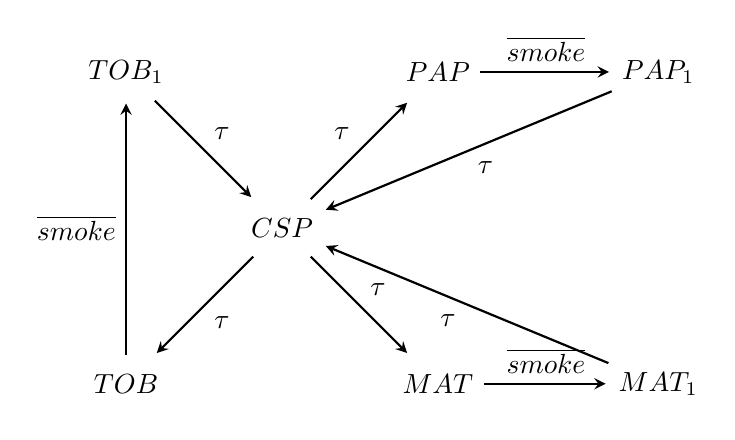
\begin{tikzpicture}[%
 	    ->,
 	    >=stealth,
 	    shorten >=1pt,
 	    node distance=2.8cm,
 	    %on grid,
 	    auto,
 	    state/.append style={minimum size=2em},
 	    thick
 	  ]
 
 
   %\tikzstyle{every state}=[fill=red,draw=none,text=white]
 
 
 	  \node[state] (CSP) {$CSP$};
 	  \node[state] (PAP) [above right of=CSP] {$PAP$};
 	  \node[state] (TOB) [below left of=CSP] {$TOB$};
 	  \node[state] (MAT) [below right of=CSP] {$MAT$};
 	  \node[state] (PAP1) [right of=PAP] {$PAP_{1}$};
    	  \node[state] (TOB1) [above left of=CSP] {$TOB_{1}$};
 	  \node[state] (MAT1) [right of=MAT] {$MAT_{1}$};

 	  \path[->] 
 	      
              (CSP)
		  edge node {$\tau$} (PAP)
		  edge node {$\tau$} (TOB)
		  edge node {$\tau$} (MAT)
 	      (PAP)
		  edge node {$\overline{smoke}$} (PAP1)
 	      (TOB)
		  edge node {$\overline{smoke}$} (TOB1)
 	      (MAT)
		  edge node {$\overline{smoke}$} (MAT1)
 	      (PAP1)
		  edge node {$\tau$} (CSP)
 	      (TOB1)
		  edge node {$\tau$} (CSP)
 	      (MAT1)
		  edge node {$\tau$} (CSP);
          
       \end{tikzpicture}
     \end{center}
  where 
 
 \begin{center}
    \begin{tabular}{l}
      $PAP \stackrel{def}{=} 
	(\nu tob,pap,mat,end)(end().Agent|S_{tob}|S_{mat}|\overline{smoke}.\overline{end}.S_{pap})$
    \\
      $TOB \stackrel{def}{=} 
	(\nu tob,pap,mat,end)(end().Agent|\overline{smoke}.\overline{end}.S_{tob}|S_{mat}|S_{pap})$
    \\
      $MAT \stackrel{def}{=} 
	(\nu tob,pap,mat,end)(end().Agent|S_{tob}|\overline{smoke}.\overline{end}.S_{mat}|S_{pap})$
    \\
      $PAP_{1} \stackrel{def}{=} 
	(\nu tob,pap,mat,end)(end().Agent|S_{tob}|S_{mat}|\overline{end}.S_{pap})$
    \\
      $TOB_{1} \stackrel{def}{=} 
	(\nu tob,pap,mat,end)(end().Agent|\overline{end}.S_{tob}|S_{mat}|S_{pap})$
    \\
      $MAT_{1} \stackrel{def}{=} 
	(\nu tob,pap,mat,end)(end().Agent|S_{tob}|\overline{end}.S_{mat}|S_{pap})$
    \\\\
    \end{tabular}
  \end{center}
\end{example}







% \begin{example}
%   This example combines both multi-party synchronization and transactional synchronization. Here we used a linear notation for derivation trees because they are too big:
% \begin{equation*}
%   \begin{fitch}
%     \fa (\underline{\overline{a}f}.\overline{b}g.P
% 	|\underline{a(w)}.a(z).Q)
% 	|\underline{b(y)}.\overline{a}h.R\; 
% 	  \xrightarrow{\tau} 
% 	    (P|Q\{f/w\})\{h/z\}|R\{g/y\}
%       & 
% 	LCom        
%     \\
%     \fa \fa \underline{\overline{a}f}.\overline{b}g.P
% 	    |\underline{a(w)}.a(z).Q
% 	      \xrightarrow{\overline{b}g\cdot a(z)} 
% 		P |Q\{f/w\}
%       &  
% 	LCom
%     \\
%     \fa \fa \fa \underline{\overline{a}f}.\overline{b}g.P
% 		  \xrightarrow{\overline{a}f\cdot \overline{b}g} 
% 		    P
%       &  
% 	SOut
%     \\    
%     \fa \fa \fa \fa \overline{b}g.P
% 		      \xrightarrow{\overline{b}g} 
% 			P
%       &  
%       Pref
%     \\    
% 
%     \fa \fa \fa \underline{a(w)}.a(z).Q
% 		  \xrightarrow{a(w)\cdot a(z)} 
% 		    Q
%       &  
% 	SInp
%     \\
%     \fa \fa \fa \fa a(z).Q
% 		      \xrightarrow{a(z)} 
% 			Q
%       &  
% 	Pref
%     \\
% 
%     \fa \fa \fa Sync(\overline{a}f\cdot \overline{b}g, a(w)\cdot a(z),\overline{b}g \cdot a(z), \{\}, \{f/w\})
%       &  
% 	S4R
%     \\
%     \fa \fa \fa \fa Sync(\overline{b}g, a(z)\{f/w\},\overline{b}g \cdot a(z), \{\}, \{\})
%       &  
% 	I3L
%     \\
%     \fa \fa \fa \fa \fa Sync(\epsilon, a(z), a(z), \{\}, \{\})
%       &  
% 	I4R
%     \\
%     \fa \fa \underline{b(y)}.\overline{a}h.R\; 
% 	      \xrightarrow{b(y)\cdot \overline{a}h}
% 		R
%       &  
% 	SInp
%     \\
%     \fa \fa \fa \overline{a}h.R\; 
% 		  \xrightarrow{\overline{a}h}
% 		    R
%       &
% 	Pref
%     \\
%     \fa \fa Sync(\overline{b}g\cdot a(z), b(y)\cdot \overline{a}h, \tau, \{h/z\}, \{g/y\})
%       &  
% 	S4R
%     \\
%     \fa \fa \fa Sync(a(z), \overline{a}h, \tau, \{h/z\}, \{g/y\})
%       &  
% 	S1L
%     \\
%   \end{fitch}
% \end{equation*}
% \end{example}
% 
% 
% \begin{example}
% \begin{equation*}
%   \begin{fitch}
%     \fa \underline{x(a)}.\overline{a}z.P
% 	|\overline{x}b.Q\; 
% 	  \xrightarrow{\overline{b}z} 
% 	    P\{b/a\}|Q
%       &
% 	LCom   
%     \\
%     \fa \fa \underline{x(a)}.\overline{a}z.P
% 	      \xrightarrow{x(a)\cdot \overline{a}z} 
% 		P
%       &  
% 	SInp
%     \\
%     \fa \fa \fa \overline{a}z.P
% 	      \xrightarrow{\overline{a}z} 
% 		P
%       &  
% 	Inp
%     \\
%     \fa \fa \overline{x}b.Q\; 
% 	      \xrightarrow{\overline{x}b} 
% 		Q
%       &  
% 	Pref
%     \\    
%     \fa \fa Sync(x(a)\cdot \overline{a}z,\overline{x}b,\overline{b}z,\{b/a\},\{\})
%       &  
% 	S3L
%     \\
%   \end{fitch}
% \end{equation*}
% \end{example}
% 





